% This is part of Un soupçon de mathématique sans être agressif pour autant
% Copyright (c) 2015
%   Laurent Claessens
% See the file fdl-1.3.txt for copying conditions.

\begin{exercice}[\cite{NRHooXFvgpp5}]\label{exo2smath-0166}

    Parmi les figures suivantes, lesquelles sont des parallélogrammes ?
    \begin{multicols}{2}
    \begin{enumerate}
        \item
           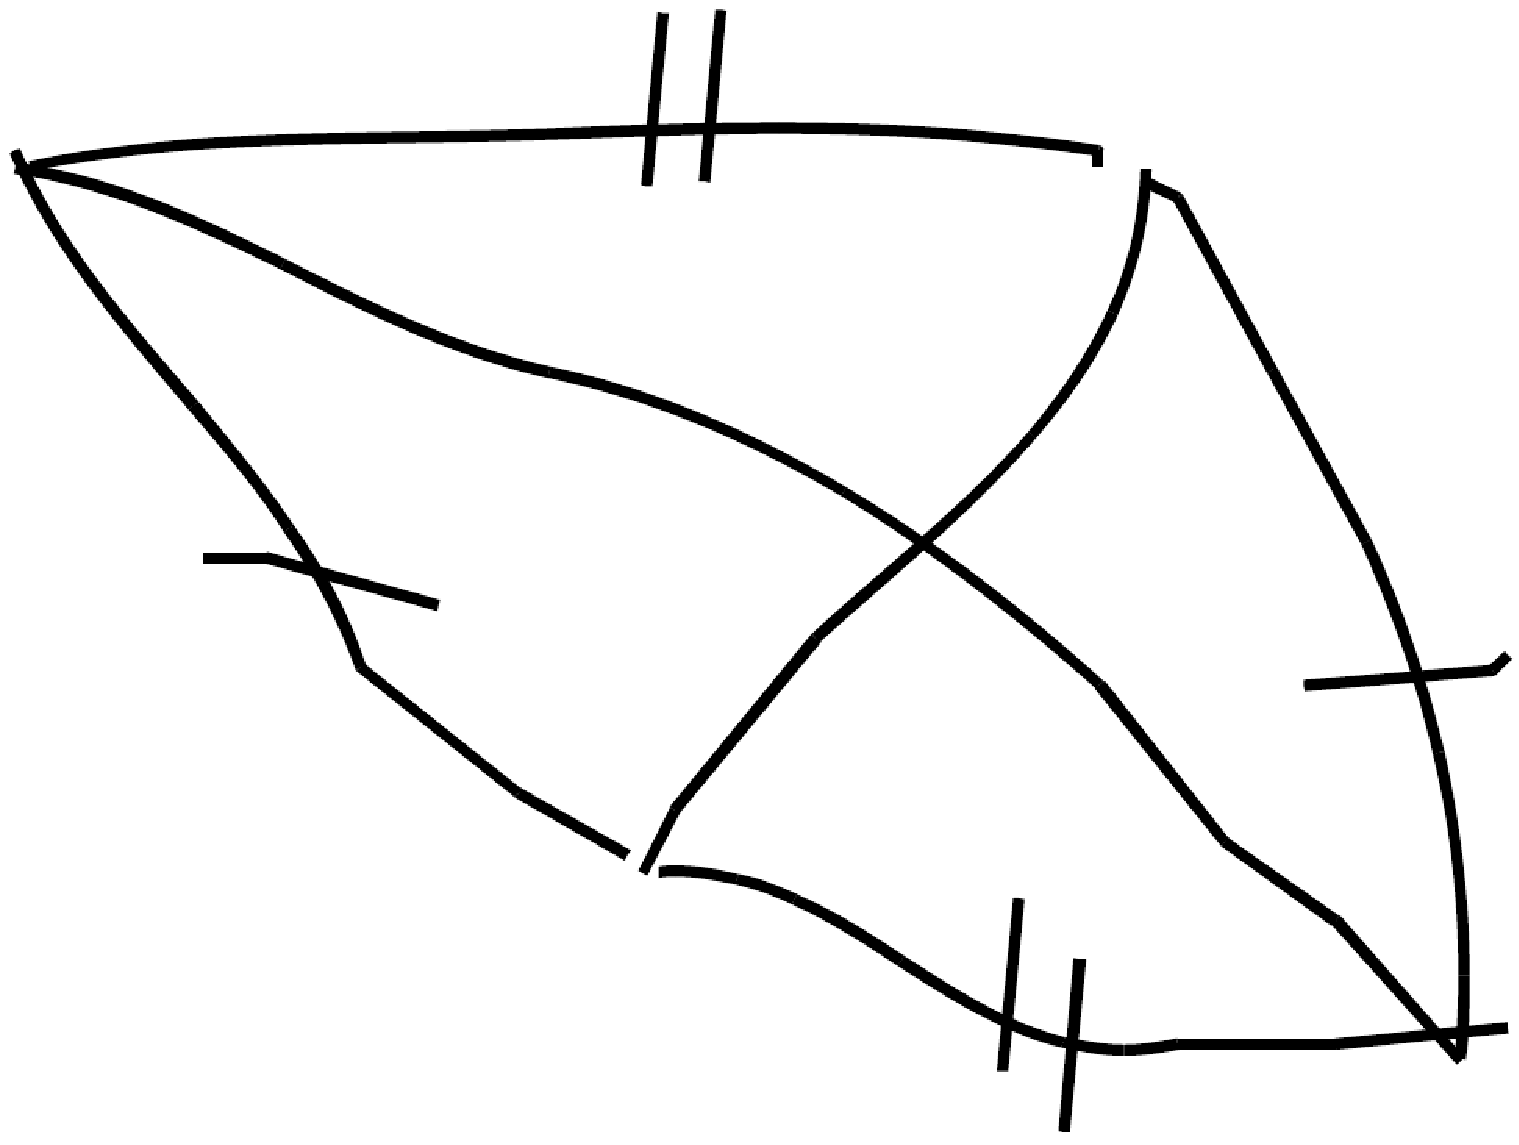
\includegraphics[width=3cm]{faux_paral1.pdf} 
        \item
           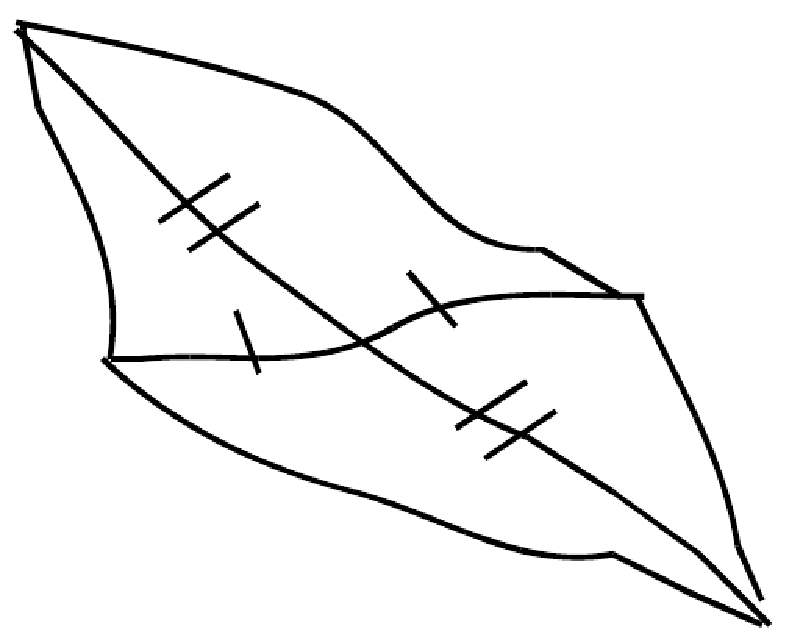
\includegraphics[width=3cm]{faux_paral2.pdf} 
        \item
           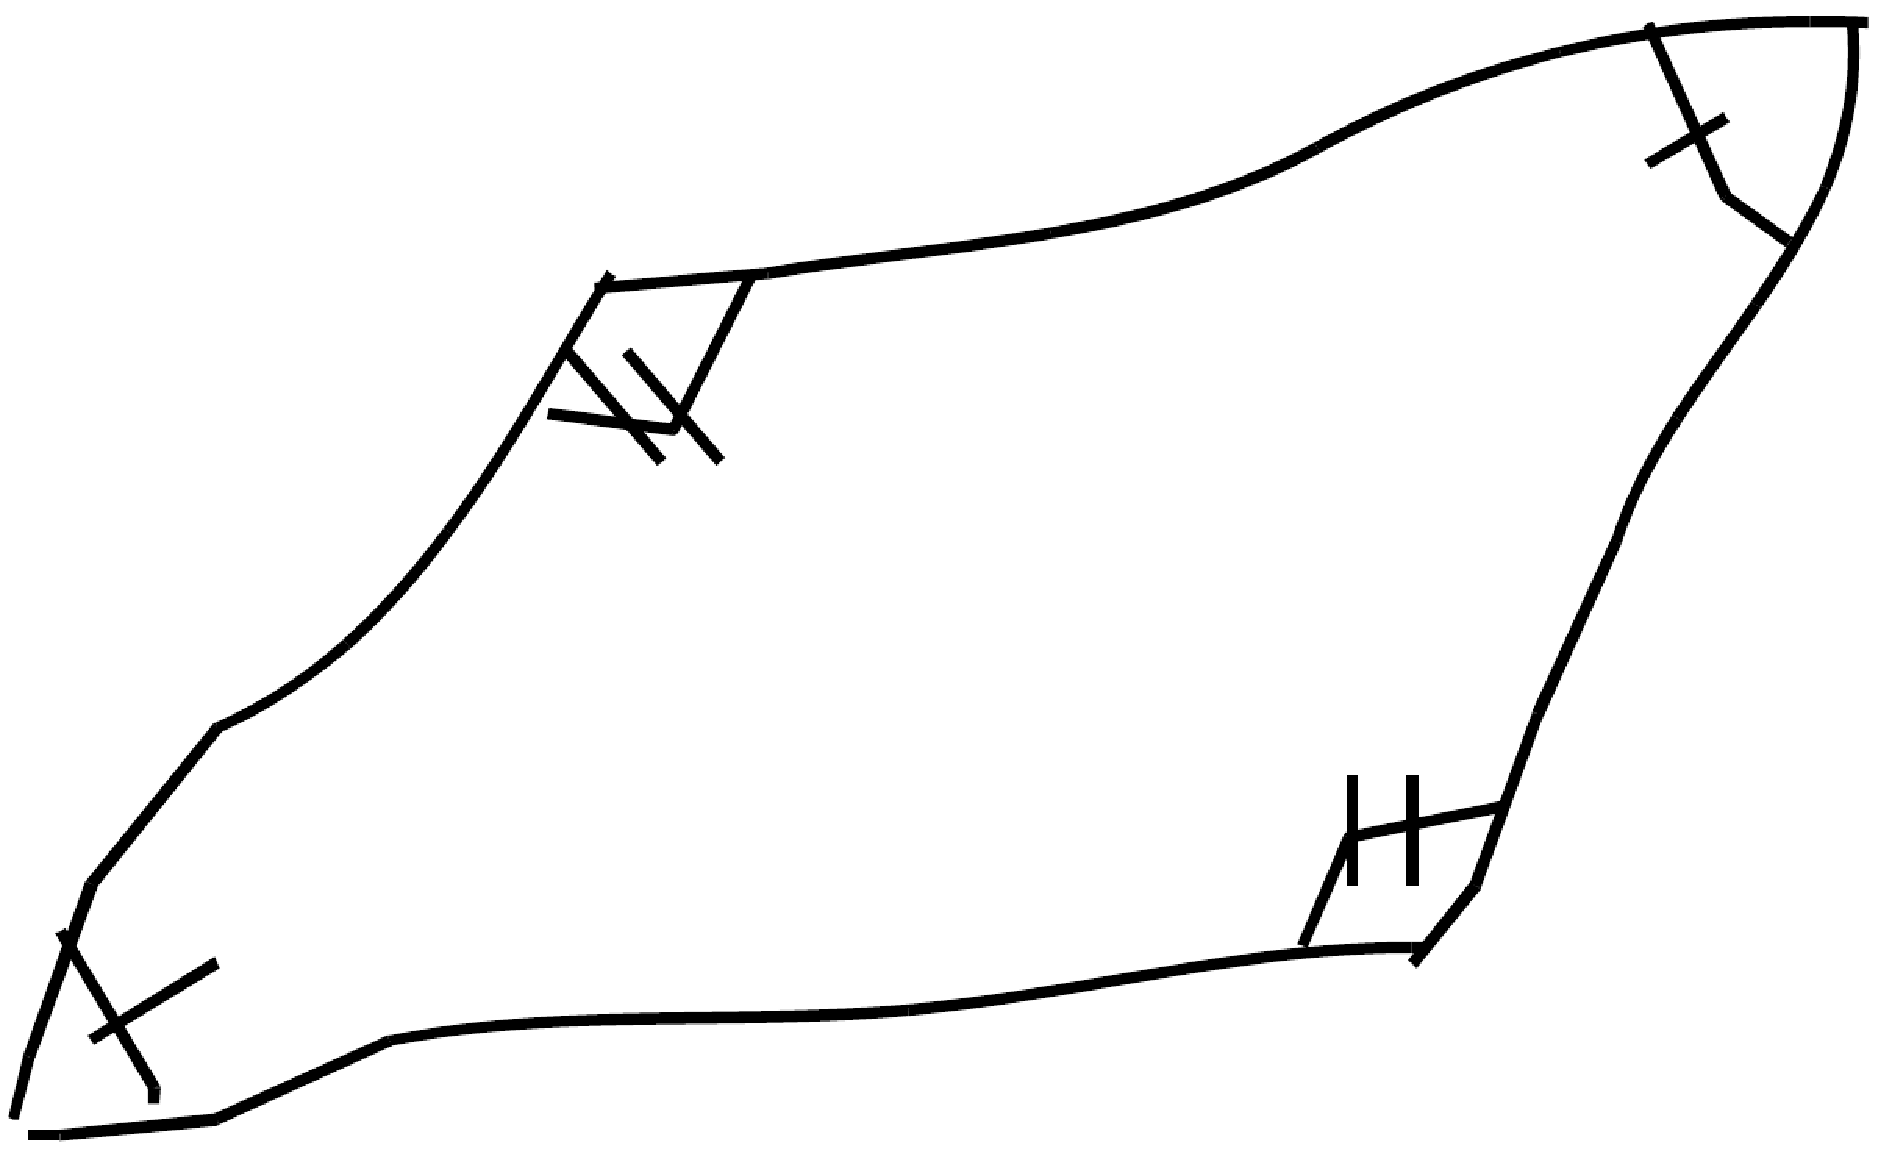
\includegraphics[width=3cm]{faux_paral3.pdf} 
        \item
           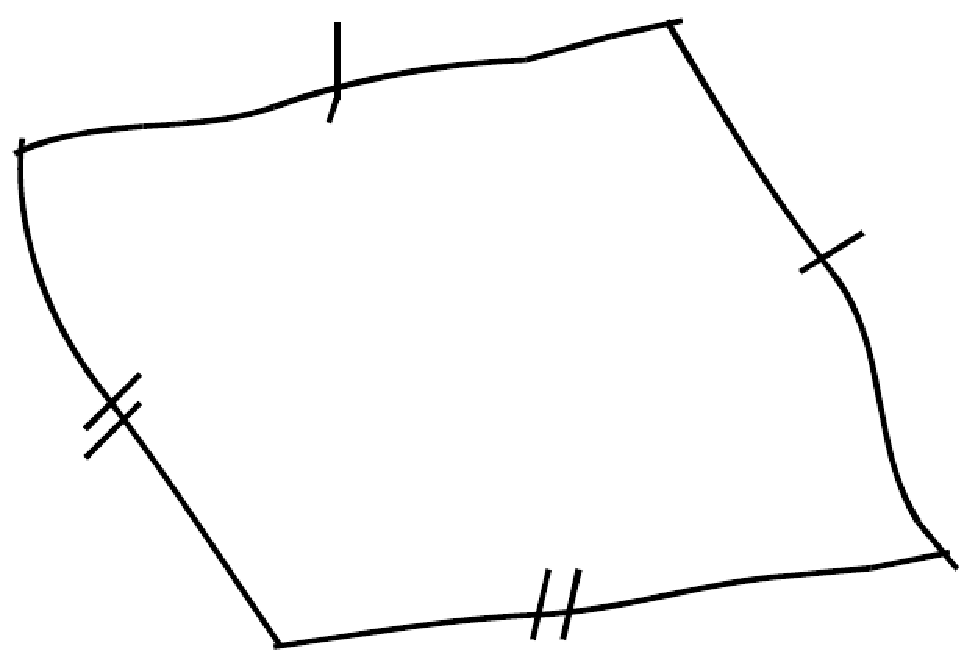
\includegraphics[width=3cm]{faux_paral4.pdf} 
    \end{enumerate}
    \end{multicols}

\corrref{2smath-0166}
\end{exercice}
